%!TEX root = ../report.tex

% 
% Architecture
% 

\section{Solution Proposal} 
\label{solutionproposal}

As referred before, it is necessary a new solution where different organizations, with different FM systems, would be able to visualize their FM results through a graphical illustration of their KPIs. The most important fact here will be the aggregation of information of different organizations, that will be compared between them, bringing a better insights where your organization is in terms of FM relatively to others. Organizations will then be ranked by their results, but their information will never be shown to others, being the results always classified.

\subsection{Overview}

The solution will be developed as a Web Application, which will be divided in two parts. Server side and Client side. The server side will run directly on the hosting servers, while the client side will run on the browser as an endpoint to the server.
The solution will:


\begin{itemize}
	\item Use authentication service to authenticate the users of a organization
	\item Display KPIs through graphics		
	\item Have a ranking between organizations
	\item Have a cache on the database for better performance
\end{itemize}

This document solution architecture overview can be found on Figure \ref{fig:architecture}. 

\begin{figure}[t!]
  \centering
  %\begin{adjustwidth}{-3cm}{0cm}
  %\begin{sideways}
  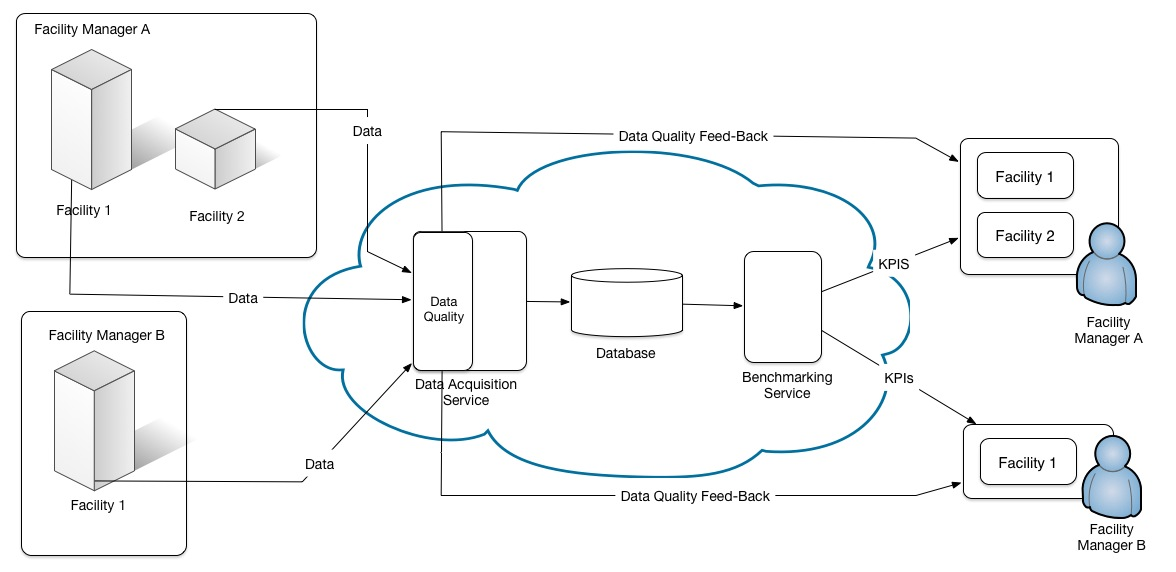
\includegraphics[width=1\textwidth]{img/OrganizacaoGeral.jpg}
  %\end{sideways}
  %\end{adjustwidth}
  \caption{FM benchmarking system architecture. Organizations send their data on a standard format, to be stored on a database. This info is then accessed by different users representatives of each organization.}
  \label{fig:architecture}
\end{figure}

\subsection{Architecture}

\begin{description}
	\item  [Client Side] The Client Side application will be running on the browser of the user connecting to the website. This application will have to display an interface so that the user can interact with the application and where the statistics about the organization will be presented. It will be used  Bootstrap Framework for the web site design which enables a quicker development and permits an adaptive front-end for mobile devices. For the generation of the graphics will be used the javascript library highcharts and if necessary the D3.js for more complex graphics.\\

	\item [Server Side] The Server Side will be running the application and will be the responsible for the processing and storage of the data sent by the Organization to the DB. It will also be responsible for organizations and users management, authentication and data management and update (CRUD - Create, Read, Update and Delete). For the Server Side will be used the Play Framework which is also responsible for the generation of HTML templates that will be sent to the Client Side.\\

	\item [Database] It will be used a relational Database (DB), that will be theoretically divided in three: Input Data Staging Area, KPI Aggregated Data and Facility Metadata as can be seen in Figure \ref{fig:db}. The Input Data Staging Area stores the data sent by the organization. The KPI Aggregated Data uses the Input Data Staging Area data to calculate the KPIs and store them.
	Without this division there would be necessary heavier queries and consequently the system would be slower. In order to deliver KPI information in real-time, the KPI Aggregated Data caches the computed information gathered by the Input Data Staging Area, making the system quicker.

	%If the KPIs would be calculated only when a client queries that specific information, it would have been a problem: when many clients asks for more heavy data queries, the system will be overloaded. Using this system of previous calculation of the KPIs, this heavy queries will be replaced for more simple queries and the calculation of each KPI will occur only once. This will not overload the system and the performance will be better.
\end{description}

\begin{figure}[t!]
  \centering
  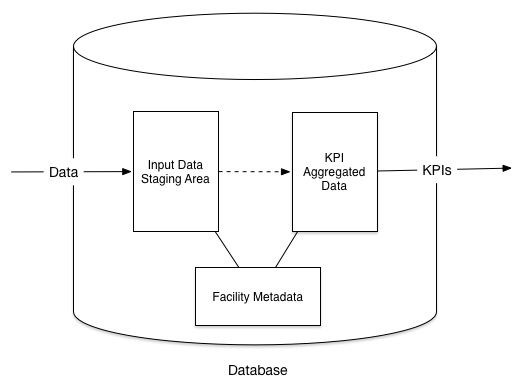
\includegraphics[width=0.70\textwidth]{img/DataBase.jpg}
  \caption{Database arrangement overview. It receives the data and stores it on Input Data Staging Area, then, when the KPIs are calculated they are stored at KPI Aggregated Data.}
  \label{fig:db}
\end{figure}

%--------------------------------------------Acabou--------------------------------
%----------------------------------------------------------------------------------
\iffalse
\begin{figure}[t!]
  \centering
  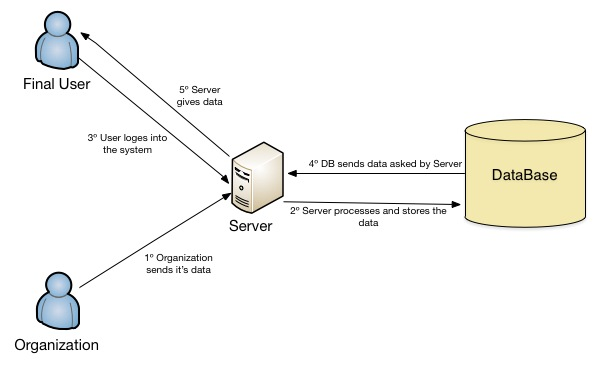
\includegraphics[width=0.95\textwidth]{img/Arquitectura.jpg}
  \caption{System Specific Architecture. }
  \label{fig:architecture}
\end{figure}

\paragraph{\bf Organization Server} \hspace{0pt} \\ The Organization Server will be a server installed on the organization. On this server each organization can subscribe the users that they want. This server will have an authenticated communication with the Central Server, and will be through it that the data will be transfered to the Central Server.

---
Organizations sends their data to the Server that is responsible for the process and store of it to the DB. Users can ask for the information stored, but for that, they have to be authenticated on the Web Application. Then, the Server asks and sends the data to the specific client.
----

\subsection{Implementation}

\begin{itemize}
	\item DB dividida dados/index
	\item que db usar?
	\item na cloud
	\item interface a utilizar
	\item que tipo de interface - o que usar?
	\item recebe dados, calcula logo os index e guarda-os
	\item Como calcular os index - kpis importantes
	\item que dados recebe e que index são calculados
\end{itemize}
\fi